\begin{figure}[!ht]
\centering
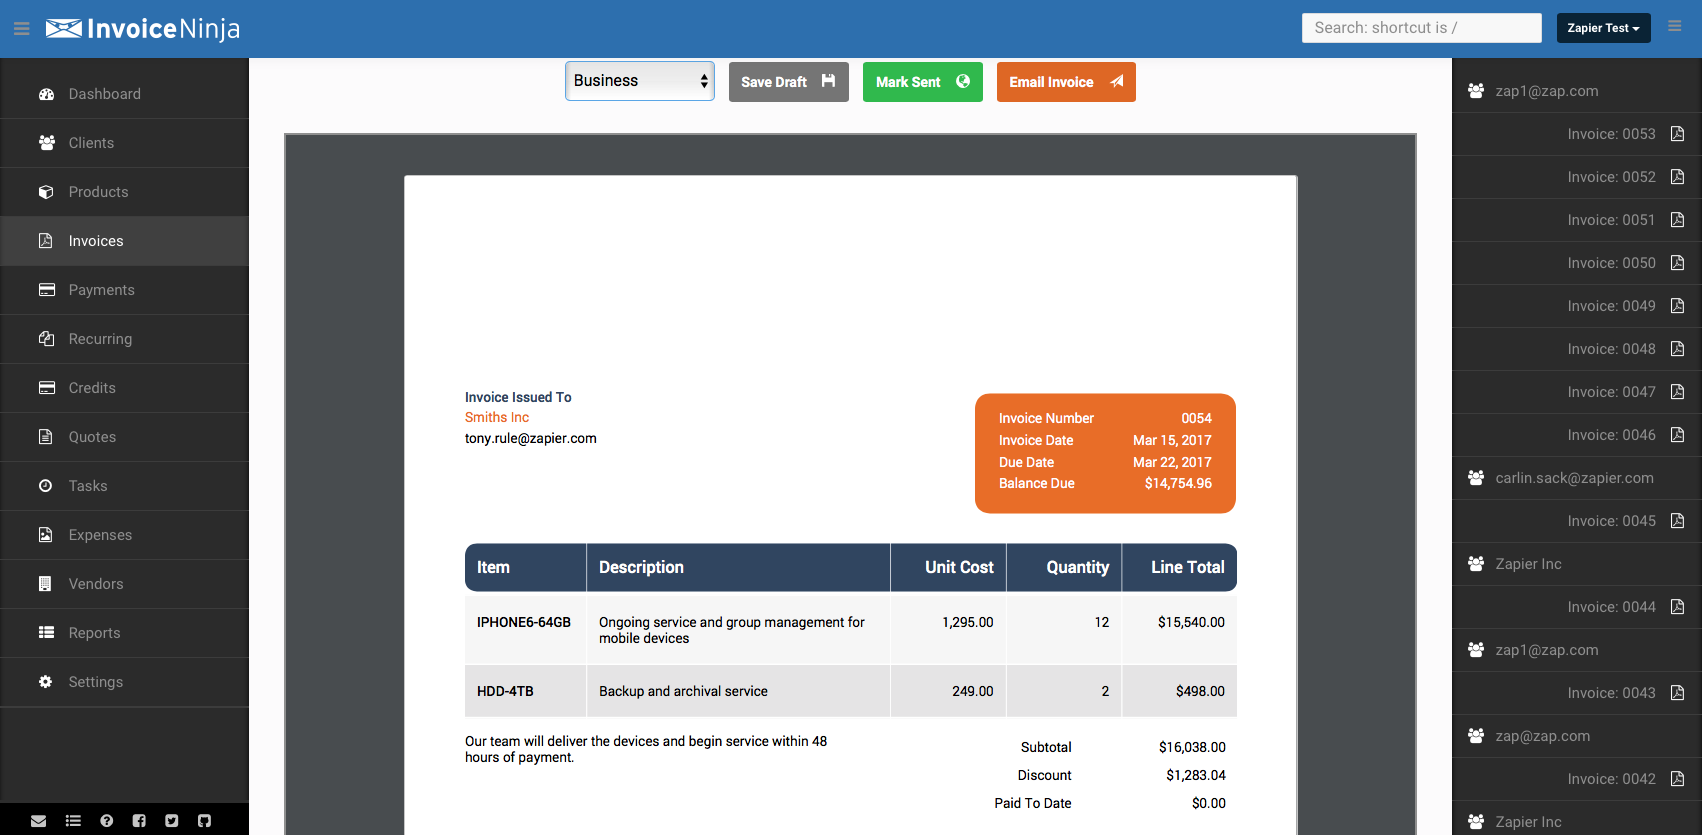
\includegraphics[width=1\textwidth]{images/5.png}                   
\caption{Dashboard}
\hspace{-1.5em}
\end{figure}
\begin{enumerate}
\item \textbf{Create Database}
\begin{itemize}
\item mysql -u root -p
\item CREATE SCHEMA `ninja` DEFAULT CHARACTER SET utf8 COLLATE utf8\_general\_ci;
\item CREATE USER 'ninja'@'localhost' IDENTIFIED BY 'ninja';
\item GRANT ALL PRIVILEGES ON `ninja`.* TO 'ninja'@'localhost';
\item FLUSH PRIVILEGES;
\item exit
\end{itemize}
\item \textbf{Configure Web Server}
\begin{itemize}
\item sudo vim /etc/apache2/sites-available/000-default.conf
\item Do the following changes:
    DocumentRoot /var/www/ninja/public\\
    <Directory /var/www/ninja/public>\\
    AllowOverride All\\
    </Directory>
\item Enable Apache rewrite mode
\begin{itemize}
 \item sudo a2enmod rewrite
\item sudo service apache2 restart
\end{itemize}
\end{itemize}
\item \textbf{Invoice Ninja Web Setup}
\begin{itemize}
\item sudo cp bootstrap/environment.default.php bootstrap/environment.php
\item sudo chown www-data:www-data -R /var/www/ninja
\end{itemize}


\end{enumerate}

